%% Example data sheet
%% Feel free to modify and use this file for any purpose, under
%% either the LaTeX Project Public License or under public domain.

% Options here are passed to the article class.
% Most common options: 10pt, 11pt, 12pt
\documentclass[10pt]{datasheet}

% Input encoding and typographical rules for English language
\usepackage[utf8]{inputenc}
\usepackage[english]{babel}
\usepackage[english]{isodate}

% tikz is used to draw images in this example, but you can
% also use \includegraphics{}.
\usepackage{tikz}
\usepackage{pgfplots}
\usepackage{circuitikz}
\usetikzlibrary{calc}

% These define global texts that are used in headers and titles.
\title{Low-Tech Graphite Sensor}
\author{M.HAHN et A.LONGEPIERRE}
\date{April 2025}
\revision{Revision 1}
\course{MOSH}
\companylogo{\hfill}

\begin{document}

\maketitle

\begin{tikzpicture}[remember picture, overlay, shift={(current page.south west)}]
    \node[anchor=north west] at (1.3,27) {
\includegraphics[height=2cm, keepaspectratio]{Cover/banner.png}};
\end{tikzpicture}

\section{Features}

\begin{itemize}
\item{Low power usage (3.3V-5V)}
\item{Low cost and low tech}
\item{Plug-in-play}
\item{Ergonomic and easily repairable}
\end{itemize}

\section{Applications}

\begin{itemize}
\item{Test findings of \it{Pencil Drawn Strain Gauges and Chemiresistors on Paper}\footnotemark{}}
\item{Applied using a transimpedance amplifier connected to the ADC of an Arduino card}
\item{Pedagogical tool for students to design and implement their own PCB design}
\end{itemize}

\section{General Description}
This innovative sensor, conceptionalized and made by students from the Applied Physics Department of INSA Toulouse, is a tool inspired by the publication 
\textit{Pencil Drawn Strain Gauges and Chemiresistors on Paper}\footnotemark[\value{footnote}]. This research paper provides a simple, cost-efficient, and highly pedagogical tool for students 
to master their skills in Physics, Electronics, and Sensor Design. The sensor presented in the publication is a simple piece of paper with a layer of graphite 
on top of it, deposited with a pencil. 

Due to the deposited graphite on the piece of paper, the electrons are able to move freely from particle to particle due to quantum tunnelling. This effect is
extremely sensitive to the slightest movement of the paper. We observe that compressing or stretching the graphite will change the resistivity of the 
sensor. 

\footnotetext{LIN, Cheng-Wei, ZHAO, Zhibo, KIM, Jaemyung et HUANG, Jiaxing, 2014. Pencil Drawn Strain Gauges and Chemiresistors on Paper. Scientific Reports. 22 janvier 2014. Vol.4, n°1, pp.3812. DOI 10.1038/srep03812.}

% Switch to next column
\vfill\break

\hspace{1pt}

\vspace{0.65cm}

\begin{figure}[h!]
	\centering
	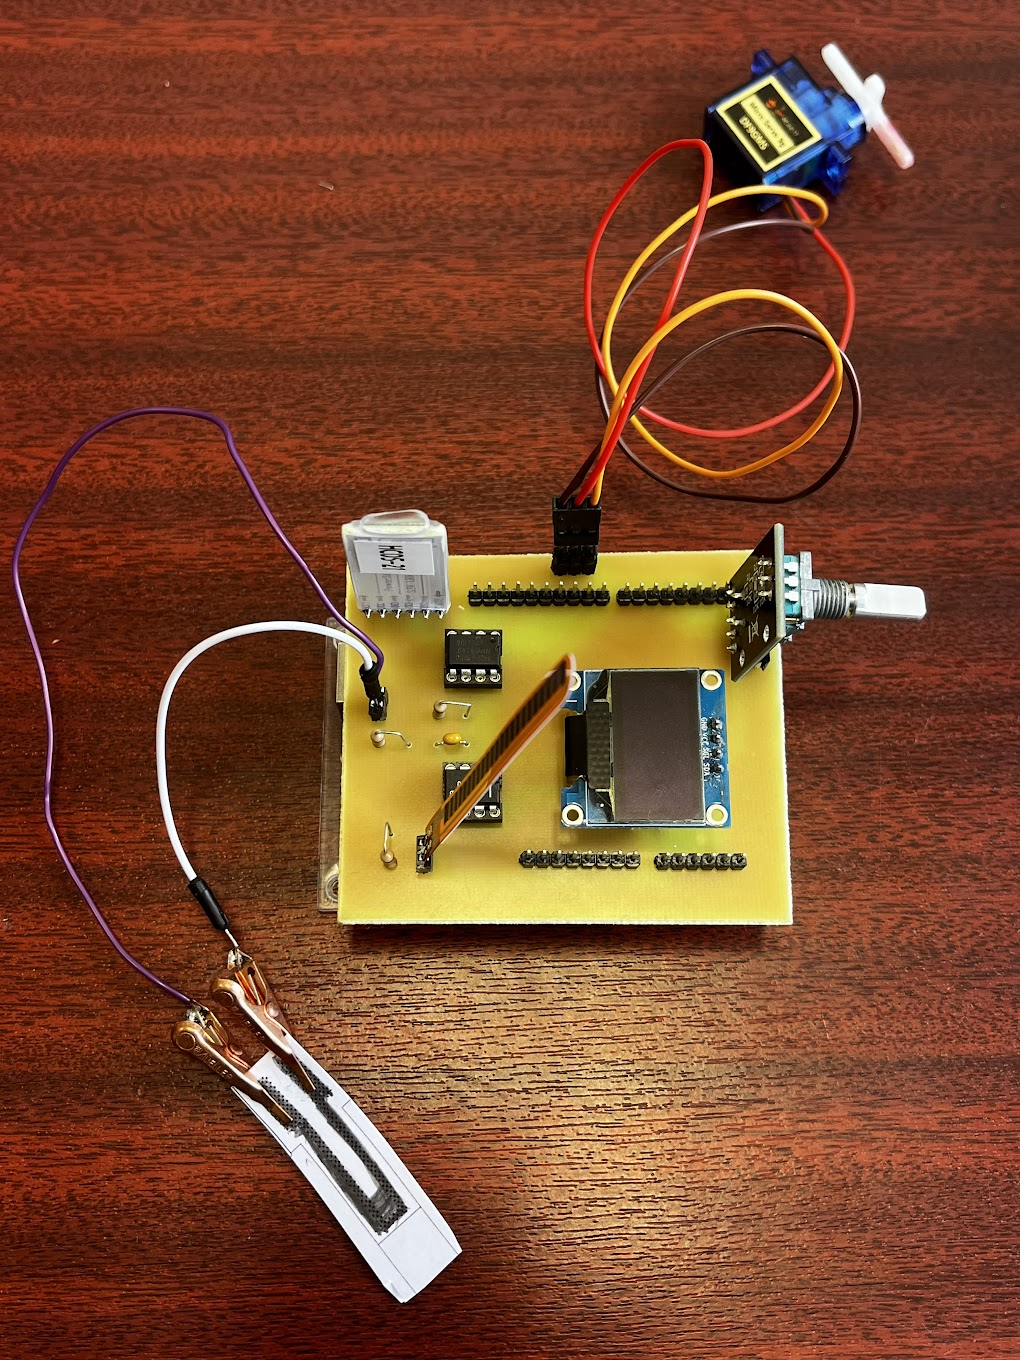
\includegraphics[width=0.3\textwidth]{Cover/PCB-Sensor.jpg}
	\caption{\small{Graphite Sensor connected to the PCB}}
\end{figure}

\vspace{1.5cm}

\begin{figure}[h!]
	\centering
	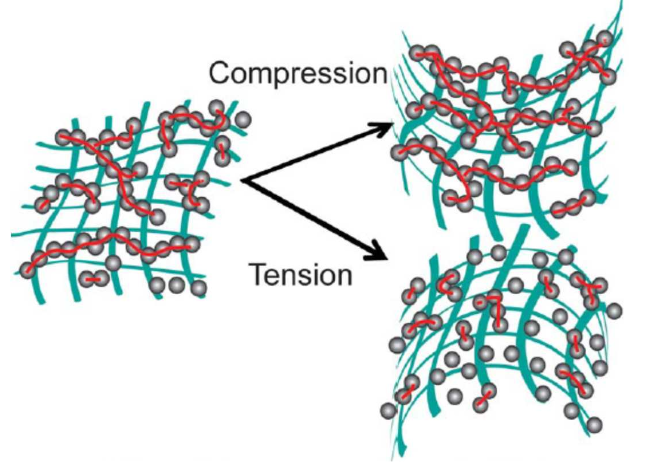
\includegraphics[width=0.3\textwidth]{Cover/Electron-Movement.png}
	\caption{\small{Compression and tension in a granular system}}
\end{figure}

% For wide tables, a single column layout is better. It can be switched
% page-by-page.
\onecolumn

\section{Electrical Diagram}

\begin{figure}[h!]
    \begin{minipage}[ts]{.47\linewidth}
        \centering
        \captionsetup{justification=centering}
        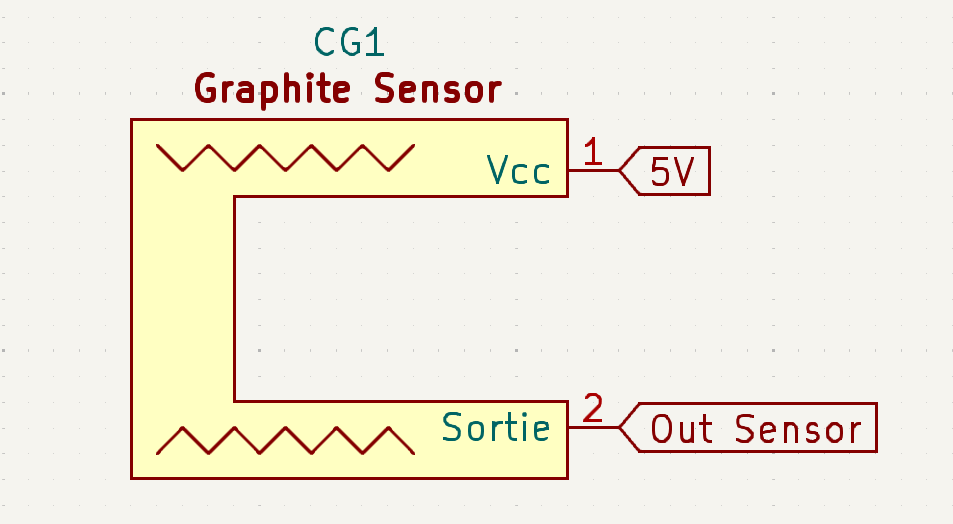
\includegraphics[width=0.8\textwidth]{Cover/ElectricDiagramSensor.png}
        \caption{\small{Schematic of the Graphite Sensor}}
    \end{minipage}
    \begin{minipage}[b]{.45\linewidth}
        \centering
        \caption*{Table 1: Specifications of the Electrical Diagram}
            \begin{tabularx}{\textwidth}{l | c | X}
                \thickhline
                \textbf{Parameter} & \textbf{Pin} & \textbf{Symbol} \\
                \hline
                Supply Voltage & V$_{\text{CC}}$ & 1 \\ 
                \hline
                Out Sensor & V$_{\text{out}}$ & 2 \\
                \thickhline
            \end{tabularx}
    \end{minipage}
\end{figure}

\setcounter{table}{1}

\section{Electrical Specifications}
All specifications are in $-40\degree C \leq T_A \leq 85\degree C$ unless otherwise noted.

\begin{table}[h]
\begin{threeparttable}
\caption{Example Data Sheet Specifications}
\begin{tabularx}{\textwidth}{l | c | c c c | c | X}
    \thickhline
    \textbf{Parameter} & \textbf{Symbol} & \textbf{Min.} & \textbf{Typ.} & \textbf{Max.} &
    \textbf{Unit} & \textbf{Conditions} \\
    \hline
    Page width  & $p_w$ & 20.9 & 21.0 & 21.1 & cm & \multirow{2}{*}{Standard A4 paper} \\
    Page height & $p_h$ & 29.6 & 29.7 & 29.8 & cm &  \\
    \hline
    Insulation voltage & $E_{max}$\tnote{1} & & 1 & & kV & \\
    \thickhline
\end{tabularx}
\begin{tablenotes}
\item[1]{Based on characterization data, not tested in production.}
\end{tablenotes}
\end{threeparttable}
\end{table}

\section{Absolute Maximum Ratings}

\begin{table}[h!]
\begin{threeparttable}
\caption{Absolute Maximum Ratings of the Graphite Sensor}
\begin{tabularx}{\textwidth}{l | c | c c c | X}
    \thickhline
    \textbf{Parameter} & \textbf{Symbol} & \textbf{Min.} & \textbf{Typ.} & \textbf{Max.} & \textbf{Unit} \\
    \hline
    Supply Voltage & V$_{\text{CC}}$ & - & 5.0 & - & V \\
    \hline
    Temperature & T & 10.0 & - & 30.0 & $^\circ$C \\
    Humitidy & - & 30 & - & 60 & \% \\
    \hline
    Paper Thickness & - & 0.15 & - & 0.30 & mm \\
    Pencil Tone\tnote{1} & - & 4B & - & 2H & - \\
    \thickhline
\end{tabularx}
\begin{tablenotes}
\item[1]{Corresponds to the US grading system.}
\end{tablenotes}
\end{threeparttable}
\end{table}

\textbf{Note:}

\newpage

\section{Applications}

\begin{figure}[h!]
	\centering
	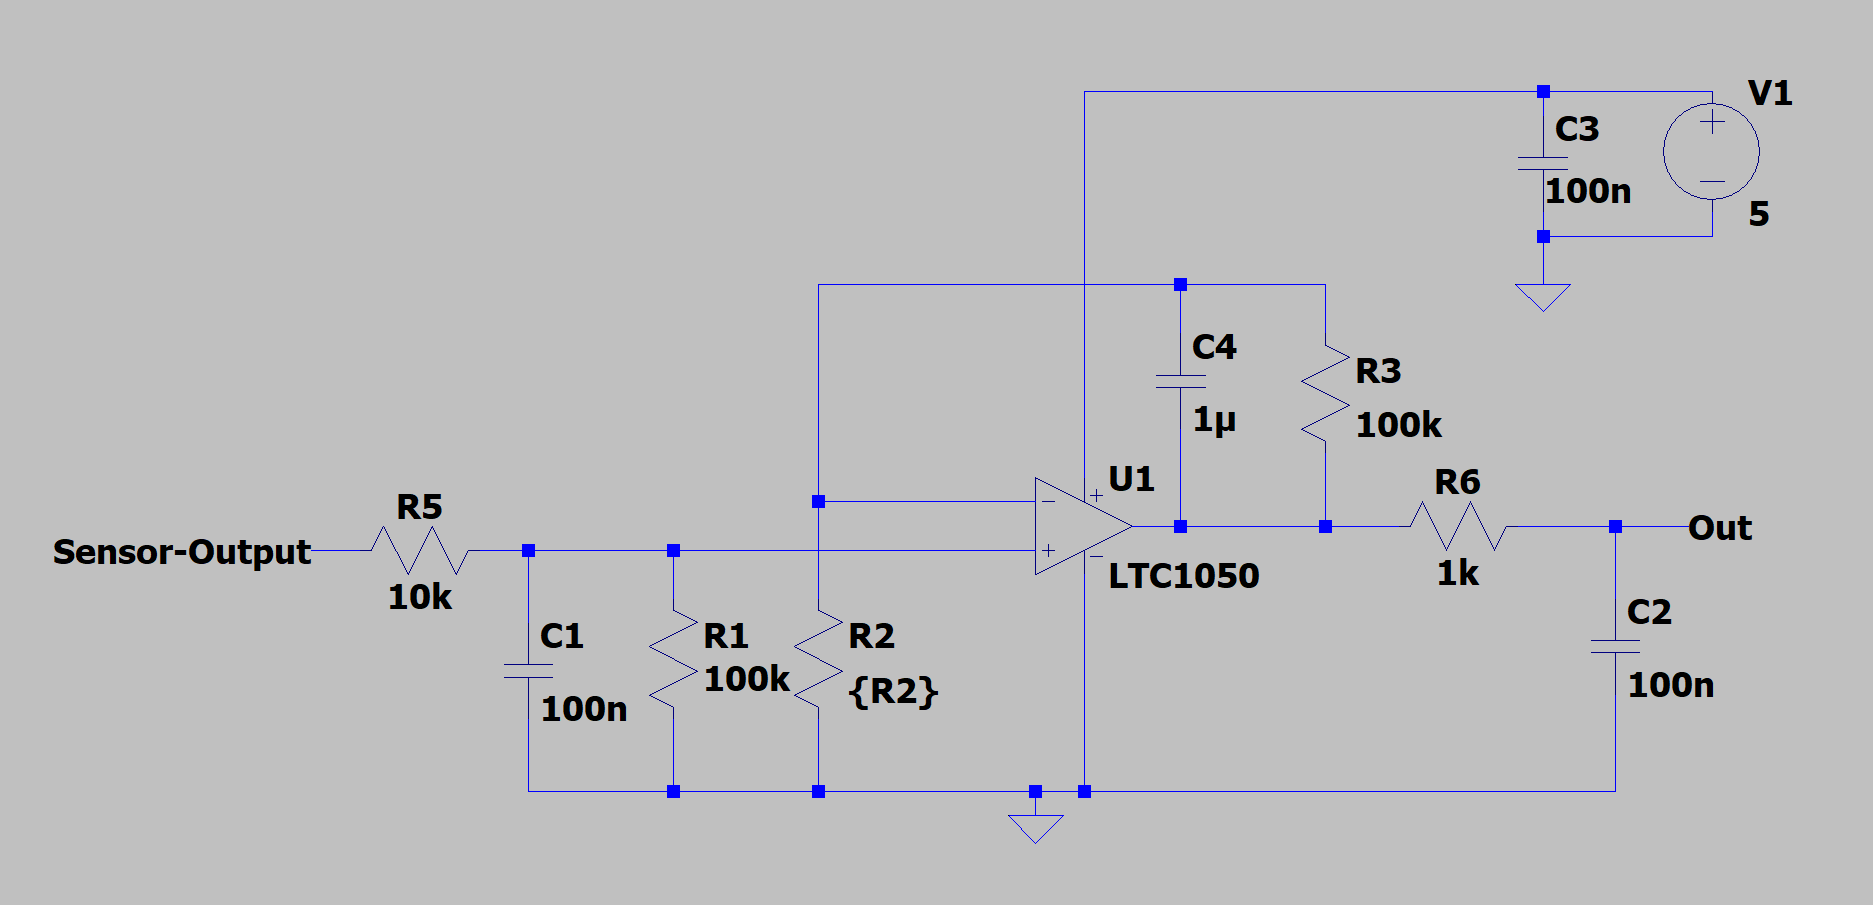
\includegraphics[width=0.6\textwidth]{Cover/TransimpedanceAmp.png}
    \captionsetup{justification=centering}
	\caption{\small{The transimpedance amplifier found on our board}}
\end{figure}

The sensor is connected to a transimpedance amplifier circuit. The circuit is equiped with a 
low-pass and high-pass filters to cancel out the noise due to the 50Hz from the sector and the amplification 
of the signal. 

The output signal of the amplifier, in our application, is transmitted to the Analog-to-digital (ADC) converter on the Arduino Uno
card. We have to make sure that the signal the ADC receives does not saturate it, thus the need for this type of amplifier. 

On our PCB, we have installed a digital potentiometer in lieu of the $\text{R}_2$ resistance in order to match the amplification of the circuit
for each pencil tone. We can calculate the value of this resistance, knowing the value of the final voltage, with the following formula :

\begin{equation*}
    R_{dp} = \frac{V_{CC}}{V_{ADC}}\times R_1\Big(1 + \frac{R_3}{R_2}\Big) - R_1 - R_5
\end{equation*}

\end{document}


